% spaTh.tex -- threshold responses with diffusion: the speed version of Theorem KBsharp.
% Input after ../JIn26/KP1 in SipArxiv.tex only; uses t:spread, t:SpdQC, r:movNGM from KP1.
\section{Threshold responses with spatial diffusion}\label{s:spaTh}
\beT[Threshold networks with diffusion keep the transition at $\bar R_0=1/L$, with a uniform speed bound]
[speed bound][SpdBd]
Let $V$, $W$, $L$, $\beta$ and $\mathcal C_L$ be as in Theorem~\ref{t:KBsharp}, with $\bar R_0=\rho(\beta WV^{-1})$, let $\mathcal D=\operatorname{Diag}(d_i)$ with $d_i>0$, and consider
\begin{equation}\label{eq:spaTh}
 x_t=\mathcal D\Delta_\zeta x-Vx+\Phi(\beta Wx),\qquad x(t,\zeta)\in\mathbb R_+^{n_S},\quad\zeta\in\mathbb R^n.
\end{equation}
\begin{enumerate}
\item If $\bar R_0<1/L$, then for every $\Phi\in\mathcal C_L$ and every $\mathcal D$, with $\bar x$ the unique equilibrium of
Theorem~\ref{t:KBsharp}, $p=(V-\beta LW)^{-1}\mathbf1$ and $c=\min_ip_i^{-1}$, every bounded nonnegative solution of \eqref{eq:spaTh} satisfies
\[
 \sup_\zeta\|x(t,\zeta)-\bar x\|_{\infty,p}\le e^{-ct}\sup_\zeta\|x(0,\zeta)-\bar x\|_{\infty,p},\qquad \|z\|_{\infty,p}=\max_i|z_i|/p_i.
\]
In particular \eqref{eq:spaTh} has no nonconstant entire solution bounded uniformly in $(t,\zeta)$, and hence no traveling front.
\item If $\bar R_0>1/L$, then for every $m\ge2$ the response of Theorem~\ref{t:KBsharp} gives, for every $\mathcal D$, at least $m$ spatially
constant, linearly exponentially stable equilibria of \eqref{eq:spaTh}.
\item Suppose that $\bar R_0>1/L$, that $\beta LW-V$ is irreducible and that $\Phi(0)=0$. Put
\[
 \bar c(L)=\inf_{\lambda>0}\frac1\lambda\,s\bigl(\lambda^2\mathcal D+\beta LW-V\bigr)>0.
\]
For every $\Phi\in\mathcal C_L$ and nonnegative, bounded, compactly supported initial data, and for every $\varepsilon>0$,
\[
 \sup_{|\zeta|\ge(\bar c(L)+\varepsilon)t}\|x(t,\zeta)\|\to0.
\]
\end{enumerate}
\eeT
\begin{proof}
(1) Let $x,y$ be two bounded nonnegative solutions and $z=x-y$. Then
$z_t=\mathcal D\Delta_\zeta z-Vz+\beta E(t,\zeta)Wz$ with $E$ diagonal and entries in $[0,L]$, a cooperative linear system. Put
$Z(t)=Ce^{-ct}p$, with $C=\sup_\zeta\|z(0,\zeta)\|_{\infty,p}$. Since $(-V+\beta EW)p\le(-V+\beta LW)p=-\mathbf1\le-cp$, both $Z-z$ and $Z+z$ are supersolutions
of that system with nonnegative initial data, so the comparison principle gives $|z|\le Z$. Taking $y\equiv\bar x$ gives the estimate. Applying it
to an entire solution from time $-T$, and letting $T\to\infty$, gives $x\equiv\bar x$.

(2) The zero-slope construction in Theorem~\ref{t:KBsharp} gives equilibria with $J=-V$. Its full-support perturbation instead gives nearby Metzler--Hurwitz Jacobians. In either case, Corollary~\ref{c:DifSta} preserves their exponential stability under every positive diagonal diffusion matrix.

(3) By the next-generation theorem, $\bar R_0>1/L$ is equivalent to $s(\beta LW-V)>0$, and Proposition~\ref{t:spread} gives a minimizer $\lambda_*$ with Perron vector
$q_*\gg0$ and $\bar c(L)>0$. Since $\Phi(0)=0$ and $\Phi'\le L$, for $x\ge0$ one has $\Phi(\beta Wx)\le\beta LWx$, so $x$ is a subsolution of the cooperative system
$u_t=\mathcal D\Delta_\zeta u+(\beta LW-V)u$. For every unit vector $e$, the function $Ce^{-\lambda_*(e\cdot\zeta-\bar c(L)t)}q_*$ solves this system and dominates the compactly supported initial data for large $C$
independent of $e$. Choosing $e=\zeta/|\zeta|$, comparison gives $\|x(t,\zeta)\|\le C'e^{-\lambda_*\varepsilon t}$ for $|\zeta|\ge(\bar c(L)+\varepsilon)t$.
\end{proof}

\beC[Diffusion preserves every constructed count of stable equilibria]
[stable equilibria under diffusion][DifSta]
Let $f$ be $C^1$ and cooperative on a convex set $K\subset\mathbb R^{n_S}$ invariant under $x_t=\mathcal D\Delta_\zeta x+f(x)$, with $\mathcal D$ a positive diagonal matrix, and let $e\in K$ be an equilibrium of $f$ with $J=Df(e)$ Hurwitz. Put $p=(-J)^{-1}\mathbf1\gg0$ and $c=\min_ip_i^{-1}$. Then
\[
 u_t=\mathcal D\Delta_\zeta u+Ju\implies\sup_\zeta\|u(t,\zeta)\|_{\infty,p}\le e^{-ct}\sup_\zeta\|u(0,\zeta)\|_{\infty,p},
\]
for bounded solutions on $\mathbb R^n$ and on bounded domains with Neumann or periodic boundary conditions, and $e$ is locally exponentially stable for the nonlinear equation in the supremum norm, for every $\mathcal D$. Consequently, at the same parameter values, the stable equilibria of Theorems~\ref{t:siphMulti}, \ref{t:KBsharp}, \ref{t:Net}, \ref{t:KBoverlapCusp} remain stable spatially constant equilibria, and the nine stable equilibria of Corollary~\ref{c:Nin} remain nine. This does not assert fronts connecting them.
\eeC
\begin{proof}
$J$ is Metzler and Hurwitz, so $-J$ is a nonsingular $M$-matrix and $Jp=-\mathbf1\le-cp$. Put $Z(t)=Ce^{-ct}p$, with $C=\sup_\zeta\|u(0,\zeta)\|_{\infty,p}$. Then $Z-u$ and $Z+u$ are supersolutions of the cooperative system $w_t=\mathcal D\Delta_\zeta w+Jw$ with nonnegative initial data, so comparison gives $|u|\le Z$, the first estimate. For a solution $x$ in $K$ near $e$, $u=x-e$ solves $u_t=\mathcal D\Delta_\zeta u+A(t,\zeta)u$, with $A=\int_0^1Df(e+\theta u)\,d\theta$ Metzler, and by continuity $Ap\le-\frac c2p$ when $\|u\|$ is small. The same comparison, with rate $c/2$, keeps $u$ small and gives the decay.
\end{proof}

\beR[What the theorem says, and a conjecture on attaining the bound]
[attaining the speed bound][SpdAtt]
The value $\bar R_0=1/L$ separates uniform attraction from possible multistability over the response class; it is not a threshold for propagation under one given response. Item 3 is an upper bound: it does not produce a wave or show that the bound is reached.

We conjecture that the bound is sharp over $\mathcal C_L$. The response $\Phi(q)=Lq/(1+Lq)$, the odds polynomial of degree one with $a_1=L$, belongs to $\mathcal C_L$, with $\Phi'(0)=L$, $\Phi''<0$ and $0\le\Phi(q)\le Lq$. Thus the linearized system at the origin is the one defining $\bar c(L)$, and $f(x)=-Vx+\Phi(\beta Wx)$ satisfies $f(x)\le(\beta LW-V)x$. If $W$ has no zero row, $f$ is cooperative, irreducible and strictly subhomogeneous, with bounded production and an unstable origin, so it has exactly one positive equilibrium, and no other equilibrium in the corresponding order interval. These are standard ingredients of linear-determinacy arguments \cite{WeinbergerLewisLi2002,Li2012}, but a direct application of the theorem of \cite{Li2012} additionally requires verification of its clipped-vector inequality: since $\beta LW-V$ is Metzler, not entrywise nonnegative, $f(x)\le(\beta LW-V)x$ does not by itself give the clipped inequality $f(\min\{\tau\xi,\bar x\})\le(\beta LW-V)\tau\xi$, $\tau>0$, of \cite{Li2012}, with $\xi$ the relevant positive eigenvector and the minimum taken componentwise.

This inequality has an exact criterion. Put $A=\beta LW-V$. For $\xi\gg0$,
\[
 f(\min\{\tau\xi,\bar x\})\le\tau A\xi\ \text{ for every }\tau>0\iff A\xi\ge0.
\]
Indeed, let $u=\min\{\tau\xi,\bar x\}$. If $u_i=\tau\xi_i$, then $f_i(u)\le(Au)_i\le\tau(A\xi)_i$, because $A$ is Metzler and the $i$th coordinates agree. If $u_i=\bar x_i$, cooperativity gives $f_i(u)\le f_i(\bar x)=0$. Conversely, for large $\tau$ all coordinates are clipped, and the inequality reads $0\le\tau A\xi$. For the Perron vector $\xi_*$ at the minimizer $\lambda_*$, $(\lambda_*^2\mathcal D+A)\xi_*=g(\lambda_*)\xi_*$, so the criterion becomes $g(\lambda_*)\ge\lambda_*^2\max_id_i$. It holds automatically for equal diffusivities, since then $A\xi_*=s(A)\xi_*\gg0$. For unequal diffusivities it can fail, so it does not establish the conjecture in general; the other hypotheses of the theorem of \cite{Li2012} also remain to be verified, and linear determinacy by another theorem is not excluded.

As a numerical illustration, take $\mathcal D=\operatorname{Diag}(1,1/10)$, $V=\begin{pmatrix}1&0\\-1/2&7/10\end{pmatrix}$,
$W=\begin{pmatrix}1/5&9/10\\3/10&1/10\end{pmatrix}$, $\beta=1$, so $\bar R_0\approx1.267$. An explicit finite-difference integration of planar fronts, which depend on $\zeta$ through one coordinate, to $t=120$ gives the speeds below;
we did not separate the part of the gap to $\bar c(L)$ due to finite time, to the grid and to the domain.
\begin{center}
\begin{tabular}{llll}
\hline
Response & $L$ & front speed & $\bar c(L)$\\\hline
$Lq/(1+Lq)$ & $2$ & $1.434$ & $1.460$\\
$1-e^{-Lq}$ & $2$ & $1.435$ & $1.460$\\
$Lq/(1+Lq)$ & $4$ & $2.390$ & $2.442$\\
$1-e^{-Lq}$ & $4$ & $2.387$ & $2.442$\\\hline
\end{tabular}
\end{center}
For these data, with $(\xi_*)_1=1$, numerically $\lambda_*\approx1.0598$ and $A\xi_*\approx(0.4236,0.8157)^\top$ for $L=2$, and $\lambda_*\approx1.6251$ and $A\xi_*\approx(1.3281,1.5727)^\top$ for $L=4$, so the clipped inequality holds in both examples.
\eeR

\beR[Related work]
[diffusion literature][SpdLit]
Adding diffusion to threshold networks is not new. The preservation of contraction under diagonal diffusion is established in \cite{AminzareSontag2012} on bounded domains with homogeneous Neumann boundary conditions, for constant diagonal weights; the comparison argument of item 1 gives the weighted maximum-norm estimate on $\mathbb R^n$. Reaction--diffusion neural networks with activation functions, $M$-matrix criteria and exponential estimates are studied in \cite{SongCaoZhao2006}, and activation-driven front initiation in nonlocal neural fields in \cite{FayeKilpatrick2018}. What is added here is that the diffusion extension preserves the sharp response-class threshold of the constructive multistability theorem, while the siphon decomposition identifies the resident-dependent transverse matrices governing linear invasion.
\eeR

\begin{figure}[H]
\centering
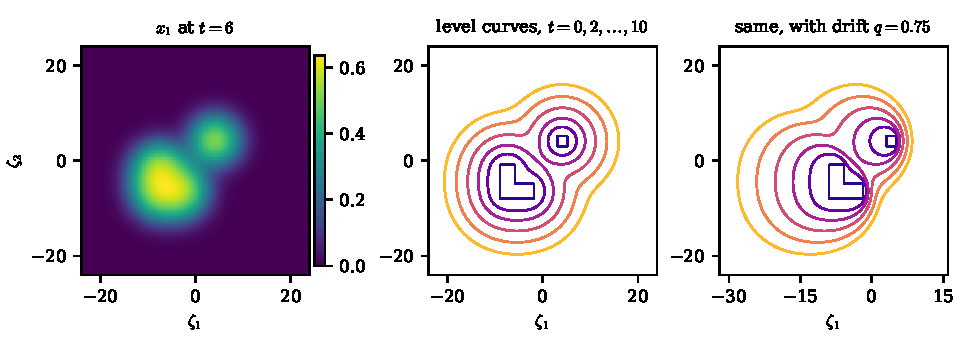
\includegraphics[width=\linewidth]{spaFront}
\caption{Fronts in the plane $\zeta=(\zeta_1,\zeta_2)$, shown without reducing to a distance from one point, by level curves of the state at successive times, for $x_t=\mathcal D\Delta_\zeta x-Vx+\Phi(Wx)$ with $\mathcal D,V,W$ of Remark~\ref{r:SpdAtt} and $\Phi(q)=2q/(1+2q)$, started from an $L$-shaped patch and a separate square.
Left: $x_1$ at $t=6$. Middle: the level curves $x_1=0.1$ at $t=0,2,\ldots,10$; the two fronts merge and the outline rounds, since the irregular initial shape fades relative to the distance travelled and the diffusion has no preferred direction. Right: the same with drift $Q=0.75\,I$
transporting toward decreasing $\zeta_1$, computed from the exact shift $x(t,\zeta)=x_0(t,\zeta+0.75\,te_1)$. At these times the outline advances at about $1.2$--$1.3$ per unit
time along the axes, below the upper bound $\bar c(2)\approx1.46$, conjectured to equal the asymptotic spreading speed.}
\label{fig:spaFront}
\end{figure}
